Here we give all results of the experiment. \Cref{fig:qbin-length-app,fig:bin-length-app,fig:no-bin-length-app} plot the \emph{ID} against the number of clicks of each game, using proportional binning, fixed size binning and no binning respectively.
\Cref{fig:qbin-time-app,fig:bin-time-app,fig:no-bin-time-app} plot the \emph{ID} against the duration of each game using proportional binning, fixed size binning and no binning respectively.

For each figure, we use the same partitioning as the graphs that are included in the paper itself.
Left: without PageRank. Right: with PageRank.
Top: `direct' semantic distance.
Top center: `graph' semantic distance.
Bottom center: graph distance.
Bottom: without distance metric.

We present these results without discussing them further.
\newpage

\begin{figure}[H]
  \centering
  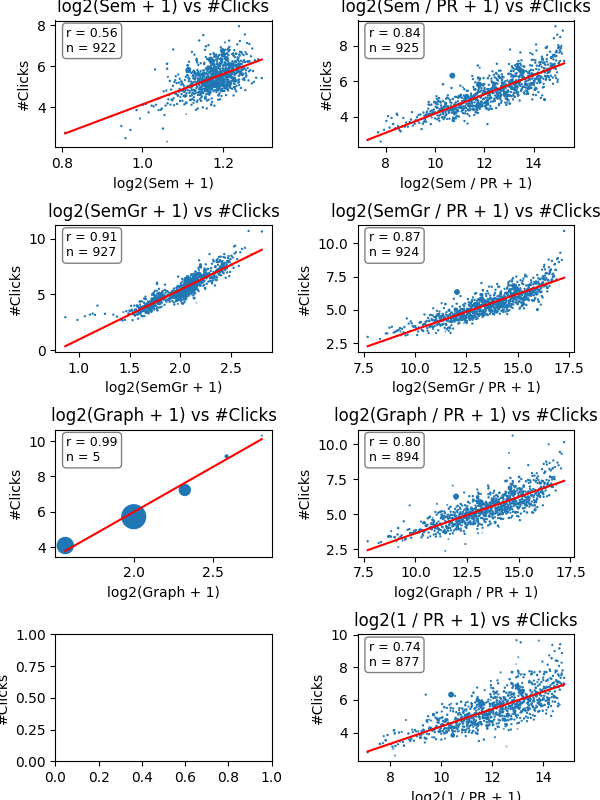
\includegraphics[width=0.82\linewidth]{../../img/qbin-Length.png}
  \caption{Number of used clicks plotted against difficulty, using various difficulty measures and proportional binning.} % \\
        %    Left: without PageRank. Right: with PageRank. \\
        %    Top: `direct' semantic distance.
        %    Top center: `graph' semantic distance.
        %    Bottom center: graph distance.
        %    Bottom: without distance metric.}
  \label{fig:qbin-length-app}
\end{figure}

\begin{figure}[H]
  \centering
  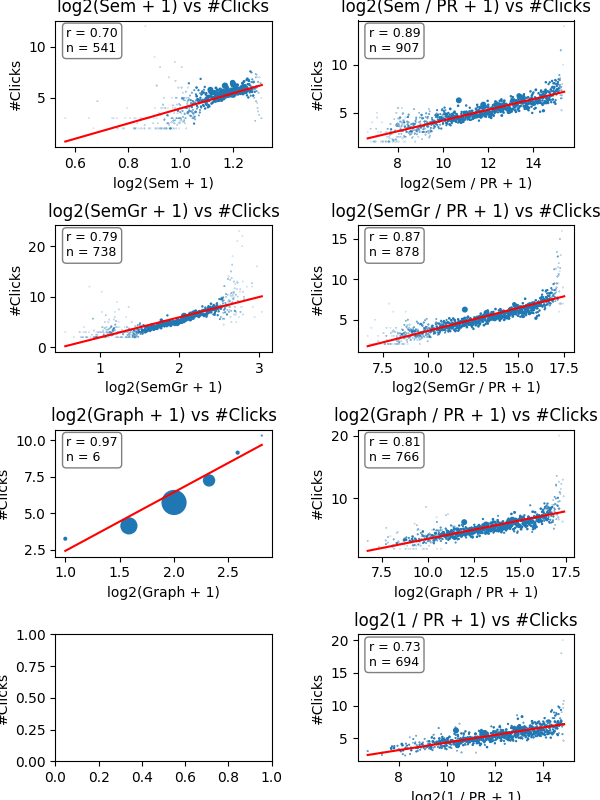
\includegraphics[width=0.82\linewidth]{../../img/bin-Length.png}
  \caption{Number of used clicks plotted against difficulty, using various difficulty measures and fixed-width binning.} % \\
        %    Left: without PageRank. Right: with PageRank. \\
        %    Top: `direct' semantic distance.
        %    Top center: `graph' semantic distance.
        %    Bottom center: graph distance.
        %    Bottom: without distance metric.}
  \label{fig:bin-length-app}
\end{figure}

\begin{figure}[H]
  \centering
  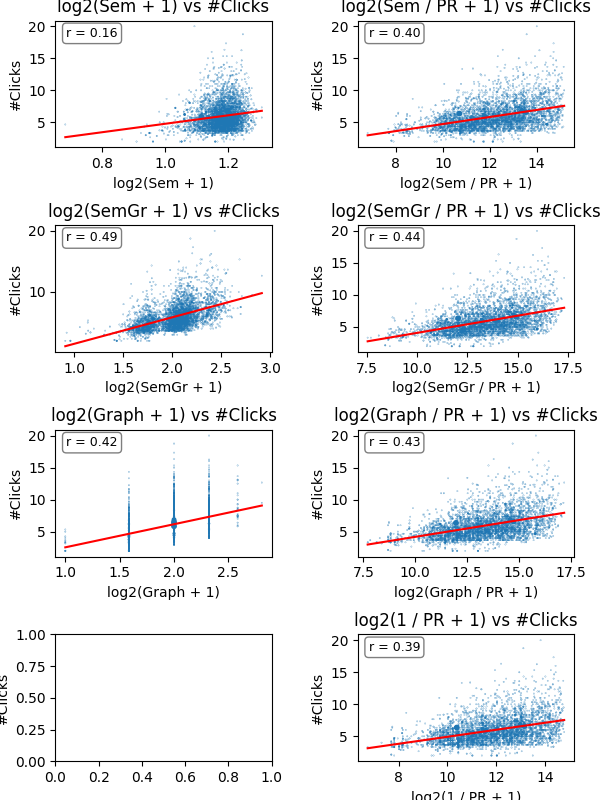
\includegraphics[width=0.82\linewidth]{../../img/nobin-Length.png}
  \caption{Number of used clicks plotted against difficulty, using various difficulty measures without any binning.} % \\
        %    Left: without PageRank. Right: with PageRank. \\
        %    Top: `direct' semantic distance.
        %    Top center: `graph' semantic distance.
        %    Bottom center: graph distance.
        %    Bottom: without distance metric.}
  \label{fig:no-bin-length-app}
\end{figure}

\begin{figure}[H]
  \centering
  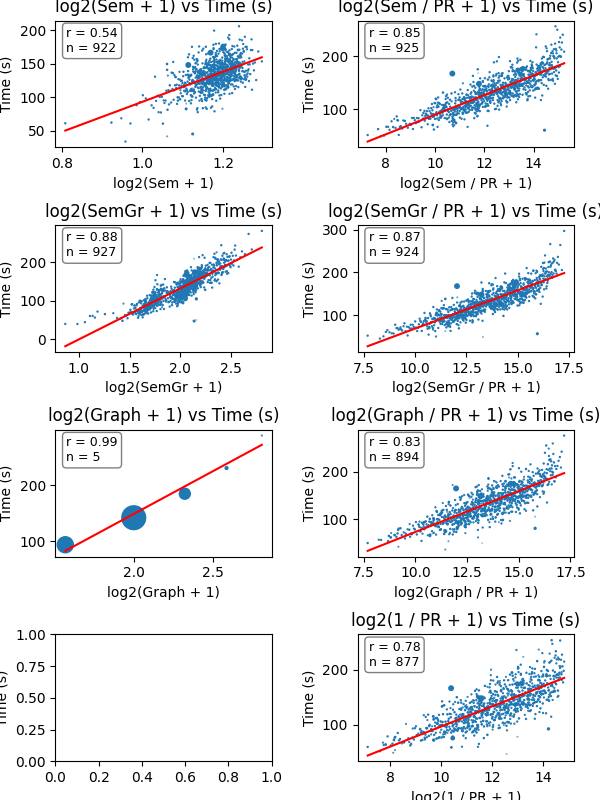
\includegraphics[width=0.82\linewidth]{../../img/qbin-Time.png}
  \caption{Duration of the game plotted against difficulty, using various difficulty measures and proportional binning.} % \\
        %    Left: without PageRank. Right: with PageRank. \\
        %    Top: `direct' semantic distance.
        %    Top center: `graph' semantic distance.
        %    Bottom center: graph distance.
        %    Bottom: without distance metric.}
  \label{fig:qbin-time-app}
\end{figure}

\begin{figure}[H]
  \centering
  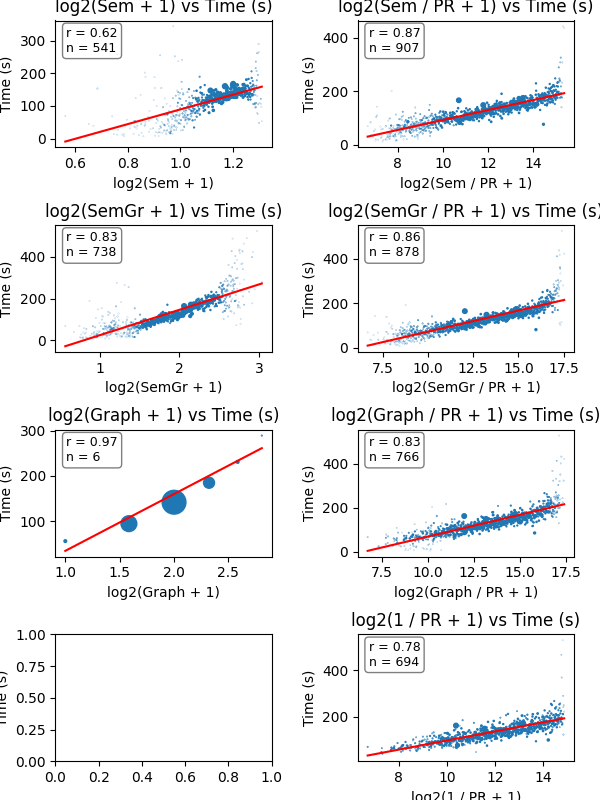
\includegraphics[width=0.82\linewidth]{../../img/bin-Time.png}
  \caption{Duration of the game plotted against difficulty, using various difficulty measures and fixed-width binning.} % \\
        %    Left: without PageRank. Right: with PageRank. \\
        %    Top: `direct' semantic distance.
        %    Top center: `graph' semantic distance.
        %    Bottom center: graph distance.
        %    Bottom: without distance metric.}
  \label{fig:bin-time-app}
\end{figure}

\begin{figure}[H]
  \centering
  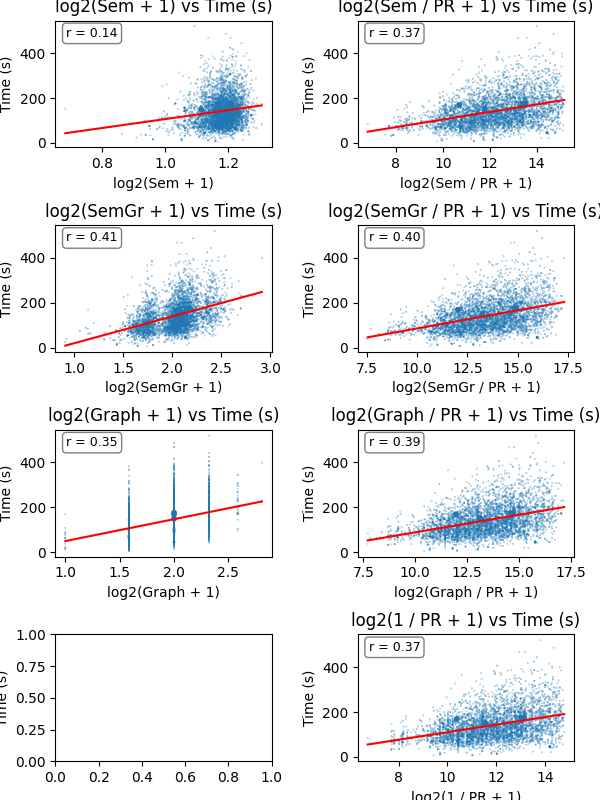
\includegraphics[width=0.82\linewidth]{../../img/nobin-Time.png}
  \caption{Duration of the game plotted against difficulty, using various difficulty measures without any binning.} % \\
        %    Left: without PageRank. Right: with PageRank. \\
        %    Top: `direct' semantic distance.
        %    Top center: `graph' semantic distance.
        %    Bottom center: graph distance.
        %    Bottom: without distance metric.}
  \label{fig:no-bin-time-app}
\end{figure}
